\pagebreak
\fontsize{12}{12}\selectfont
%\vspace{-25mm}
\section{Selecci�n de la herramienta para Data Discovery}
%\vspace{-25mm}
Fueron analizados los estudios de Gartner\cite{herschel2015magic}\cite{sallam2015critical} para la selecci�n de la mejor herramienta que se adecue a los criterios necesarios para ser utilizado en esta tesis. Estos documentos realizan un an�lisis de las mejores herramientas del mercado, en un �rea de conocimiento. A continuaci�n se presenta el Cuadrante M�gico de Gartner, para herramientas de BI y Analytics.


%\vspace{-40mm}
\section{Cuadrante M�gico de Gartner}

\textsc{\begin{figure}[H]
	\centering
	\caption{Cuadrante M�gico para BI y Plataformas Anal�ticas}
	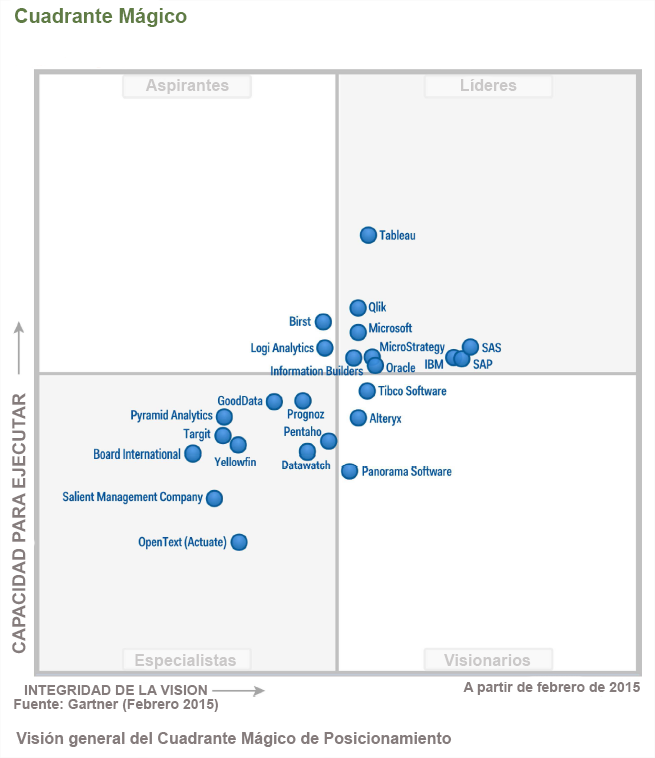
\includegraphics[width=160mm]{Magic-Quadrant.png}
	\caption*{Fuente: \citeauthor{herschel2015magic} \citeyear{herschel2015magic}}
	\label{fig:magicQuadrant}
\end{figure}}

%\subsection{Tableau}
%Tableau tiene una posici�n fuerte en capacidad de ejecuci�n en el eje de l�deres del cuadrante. Esta herramienta fue la que mejor se adecu� a las necesidades del trabajo de Tesis, dado que cuenta con una versi�n p�blica para la construcci�n y publicaci�n de dashboards, adem�s de la facilidad de uso que nos proporciona. Tableau Desktop, la cual se basa en tecnolog�a drag and drop (arrastrar y soltar) permite analizar datos r�pidamente y permite ver los cambios en tiempo real sin necesidad de codificaci�n, de esta manera, posibilita a un usuario con no muchos conocimientos t�cnicos poder utilizarlo con mayor facilidad.

\noindent
Los l�deres del mercado se encuentran siempre en el cuadrante superior derecho. Se puede observar una amplia diferencia entre Tableau y los dem�s l�deres.\\
En las siguientes figuras se presenta el an�lisis de Gartner que eval�a las capacidades cr�ticas que debe tener una herramienta de BI y Analytics, para adecuarse a las necesidades del mercado.

\textsc{\begin{figure}[H]
	\centering
	\caption{Puntuaciones de producto o servicio para an�lisis descentralizado }
	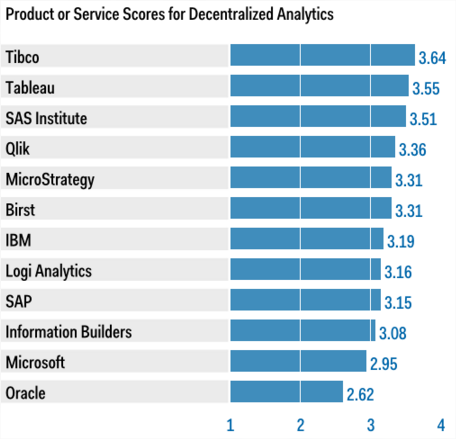
\includegraphics[width=160mm]{productOrServiceScoresForDecentralizedAnalytics.png}
	\caption*{Fuente: \cite{parenteau2015rise}}
	\label{fig:productOrServiceScoresForDecentralizedAnalytics}
\end{figure}}

\textsc{\begin{figure}[H]
	\centering
	\caption{Puntuaciones de producto o servicio guiados por Data Discovery}
	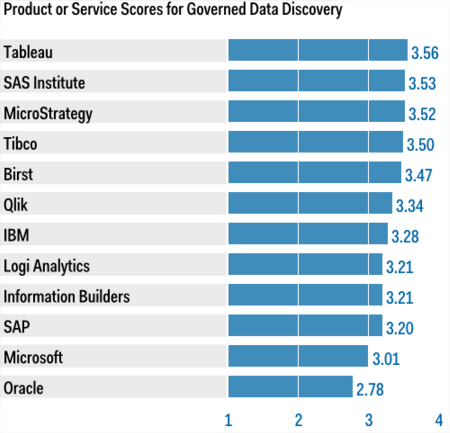
\includegraphics[width=160mm]{productOrServiceScoresForGovernedDataDiscovery.png}
	\caption*{Fuente: \cite{parenteau2015rise}}
	\label{fig:productOrServiceScoresForGovernedDataDiscovery}
\end{figure}}

\noindent
Los valores posibles van del 1 al 5, conforme la siguiente evaluaci�n:

\begin{enumerate}
	\item Pobre o ausente: la mayor�a de los requisitos de esta capacidad no fueron alcanzadas.
	\item Justo: Algunos de los requisitos fueron alcanzados.
	\item Bueno: cumple con los requisitos.
	\item Excelente: alcanza o excede algunos requisitos.
	\item Superior: excede significativamente los requisitos.
\end{enumerate}
\noindent
Tableau tiene una posici�n fuerte en capacidad de ejecuci�n (producto/servicio, su oferta, ejecuci�n de ventas, marketing, experiencia del cliente) en el eje de l�deres del cuadrante. Esta herramienta fue la que mejor se adecu� a las necesidades del trabajo de Tesis, dado que cuenta con una versi�n p�blica para la construcci�n y publicaci�n de dashboards, adem�s de la facilidad de uso que nos proporciona. Tableau Desktop, la cual se basa en tecnolog�a drag and drop (arrastrar y soltar) permite analizar datos r�pidamente y permite ver los cambios en tiempo real sin necesidad de codificaci�n, de esta manera, posibilita a un usuario con escasos conocimientos t�cnicos, poder utilizarlo de igual manera.

\textsc{\begin{figure}[H]
	\centering
	\caption{Arrastre el campo pa�s para el campo desplegable se�alado.}
	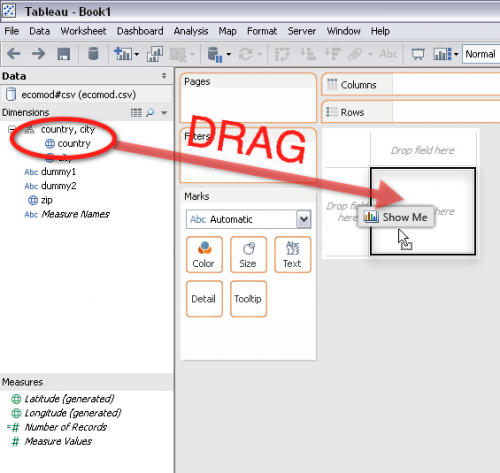
\includegraphics[width=0.7\linewidth]{imagenes/tableauDragAndDrop2}
	\caption*{Fuente: \cite{peck2013tableau}}
	\label{fig:tableauDragAndDrop2}
\end{figure}}

\textsc{\begin{figure}[H]
	\centering
	\caption{Arrastrar hojas de trabajo al dashboard.}
	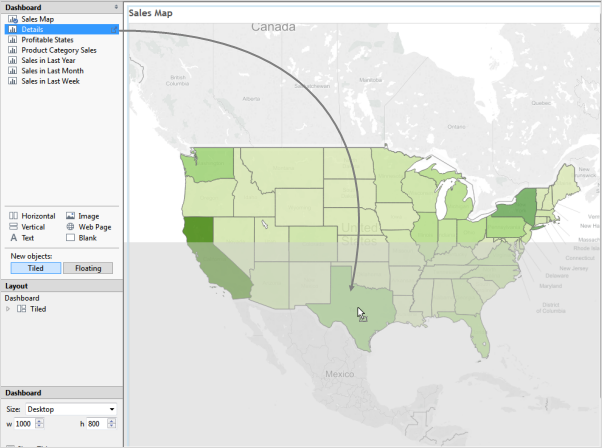
\includegraphics[width=0.7\linewidth]{imagenes/tableauDragAndDrop1}
	\caption*{Fuente: \citeauthor{peck2013tableau} \citeyear{peck2013tableau}}
	\label{fig:tableauDragAndDrop1}
\end{figure}}

\noindent
De una forma �gil el usuario puede conectarse a diversas fuentes de datos y crear paneles interactivos, conectando entre s� los diferentes componentes (tipo de gr�fico) que proporciona la herramienta. La herramienta permite utilizar componentes como filtros, siendo o no de la misma fuente de datos siempre y cuando los datos coincidan en los diversos conjuntos.
Pueden ser utilizadas en la organizaciones para comprender r�pidamente diferentes aspectos del negocio. Tambi�n se puede utilizar para realizar proyecciones o tendencias,  la cual Tableau nos ofrece de manera autom�tica.
